\documentclass{article}

\usepackage[utf8]{inputenc}
\usepackage[T1]{fontenc}
\usepackage{geometry}
\usepackage{graphicx}
\usepackage{subcaption}
\usepackage{amsmath,amssymb}
\usepackage{amstext}
\usepackage{verbatim}
\newcommand{\angstrom}{\text{\normalfont\AA}}
\usepackage{enumitem} %PERMETTE L'USO DI ELENCHI NUMERATI
\usepackage[section]{placeins}


\geometry{a4paper}

\usepackage[italian,english]{babel}
\frenchspacing

\title{Relazione sull'interferometro di Michelson}
\author{Lorenzo Ramella, Alessandro Matteo Rossi, Marco Tambini}
\date{\today}

\begin{document}
\maketitle

\begingroup
\selectlanguage{english}
\begin{abstract}
In questa esperienza abbiamo utilizzato l'interferometro di Michelson per misurare la lunghezza d'onda di un laser e, grazie a quest'ultima, l'indice di rifrazione dell'aria; successivamente abbiamo misurato la lunghezza di un pacchetto di luce bianca e abbiamo calcolato la differenza tra le due frequenze emesse da una lampada al sodio.

Riportiamo qui sotto i risultati:
\[ \lambda_{laser} = 0,619 \pm 0,016 \; \mu m \]
\[ n_{aria} = 1,000255 \pm 7 \cdot 10^{-6} \]
\[ L_{pacchetto} = 7,5 \pm 2,8 \; \mu m \]
\[ \Delta \lambda_{Na} = 6,285 \pm 0,007 \; \textrm{Å} \]

L'esperimento è stato svolto da Tambini, mentre Ramella e Rossi hanno contribuito all'analisi dei dati e alla stesura della relazione.
\end{abstract}
\endgroup

\selectlanguage{italian}
\tableofcontents



\section{Progettazione dell'esperienza}
Le sorgenti di luce usate per questo esperimento sono un laser, posizionato su una rotaia allineata con la parte "centrale" dell'apparato, una lampada al sodio (Na) e una lampada ad incandescenza. La rotaia è stata necessaria anche per posizionare la lente dispersiva per le misure del laser e la fibra ottica da attaccare alle altre lampade per indirizzarne la luce, non essendo posizionabili sulle rotaie.

%immagine apparato
\begin{figure}[h!]
  \centering
  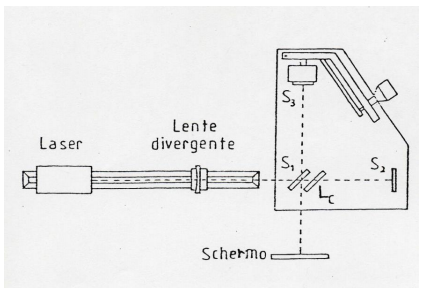
\includegraphics[width=0.7\linewidth]{IM percorso luce}
  \caption{Schema dell'apparato sperimentale. La linea tratteggiata indica il percorso della luce}
\end{figure}

\vspace{3mm}

La parte centrale dell'apparato, schematizzata in Figura 1, è formata da uno specchio semiriflettente $S_1$, uno specchio $S_3$ mobile lungo la propria normale, uno specchio $S_2$ di cui possiamo modificare l'inclinazione, una lastra compensatrice $L_C$ e una camera a vuoto removibile necessaria per le misure dell'indice di rifrazione dell'aria. 

\vspace{3mm}

La visualizzazione dei risultati è avvenuta su due schermi: uno fisso situato in lontananza e uno mobile situato in prossimità dell'apparato (il foglio di carta in Figura 2).

\vspace{2mm}

%immagine apparato
\begin{figure}[h!]
  \centering
  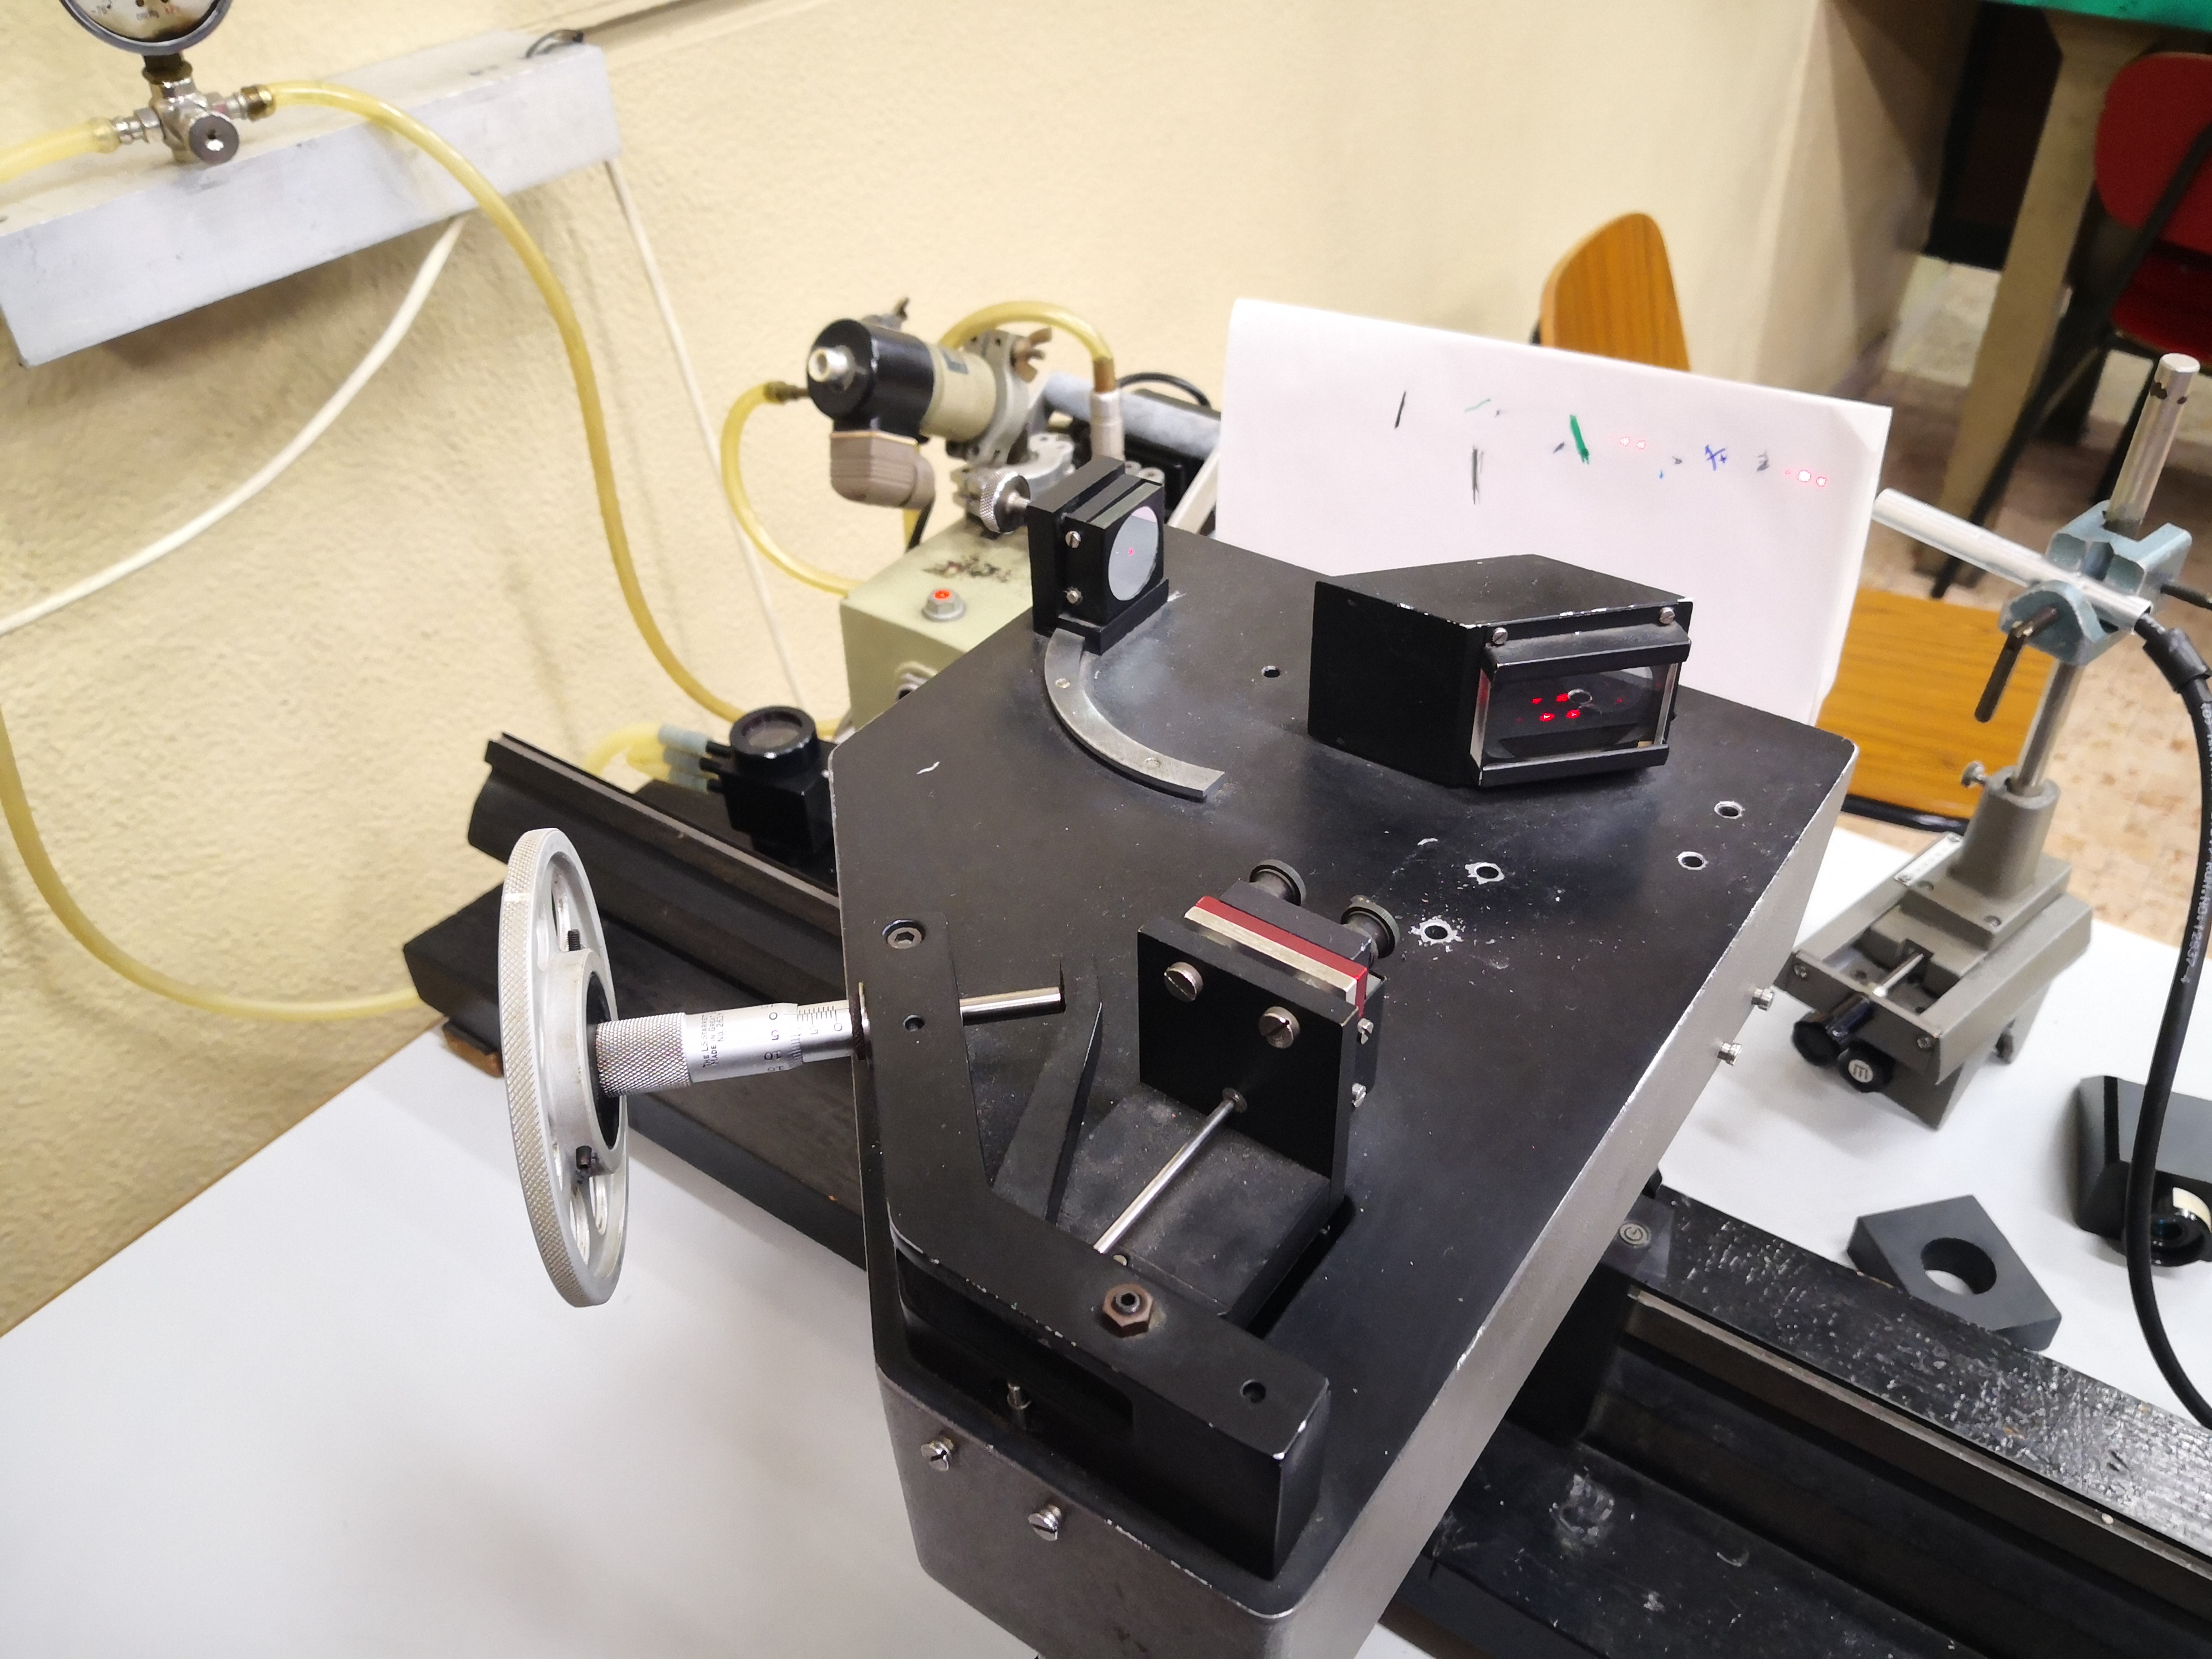
\includegraphics[width=0.5\linewidth]{IM strumentazione}
  \caption{Foto dell'apparato sperimentale}
\end{figure}



La presa delle misure è stata effettuata tramite un calibro palmer con una sensibilità di $0,01 \; mm$. Il calibro è tuttavia collegato allo specchio da una leva che riduce di 1/5 lo spostamento. Abbiamo quindi usato un'incertezza sulle misure di lunghezza pari a $2 \sqrt2 \; \mu m$.
% uso paint per scrivere cosa sono le varie cose? se si devo installarlo e reimparare ad usarlo




\section{Introduzione teorica}
\subsection{Richiami teorici}
Il fenomeno che possiamo osservare con l'apparato finora descritto è quello dell'interferenza.

Per potere osservare delle figure di interferenza stabili abbiamo bisogno di due fattori: i raggi luminosi che causano interferenza devono avere una differenza di fase costante e la loro intensità deve essere simile. Se si verificano le condizioni sopradescritte possiamo osservare due tipi principali di interferenza:

Interferenza costruttiva, visibile come zone luminose, se:
\[ \Delta \phi = 0 \rightarrow I = 4 I_0 \]

Interferenza distruttiva, visibile come zone scure, se: 
\[ \Delta \phi = \pi \rightarrow I = 0 \]

L'interferenza si applica tuttavia solo in casi di onde sinusoidali infinite, non ottenibili sperimentalmente dati i tempi di emissione finiti. La presenza di tempi finiti implica un troncamento dell'onda sinusoidale. La sezione troncata viene definita pacchetto d'onda. Viene quindi definito l'intervallo di tempo $\Delta t_c$, detto tempo di coerenza, nel quale l'onda si mantiene sinusoidale e può essere considerata un'onda sinusoidale infinita. Al tempo di coerenza possiamo quindi associare una lunghezza di coerenza $L_c$ corrispondente allo spazio percorso durante il tempo di coerenza dalla luce nel vuoto.

La lunghezza di coerenza è maggiore nei casi in cui i pacchetti siano emessi in maniera coerente, come nel laser, o in cui si abbia una luce monocromatica, situazione simile alla lampada al sodio, mentre risulta drasticamente minore in casi di luce non coerente, come nel caso della luce bianca.


\subsection{Percorso della luce}


Nel suo percorso la luce incontra inizialmente la lastra semiriflettente $S_1$, incidendo su di essa il fascio si divide in due: un primo fascio prosegue indisturbato verso lo specchio $S_2$ e, dopo essere tornato indietro, viene riflesso da $S_1$ sullo schermo. Il secondo fascio viene invece riflesso, ripercorre nuovamente la lastra $S_1$ e viene riflesso da $S_3$, a questo punto attraversa nuovamente $S_1$ arrivando infine sullo schermo. La lastra di compensazione è un pannello di spessore, materiale e inclinazione uguali a $S_1$ in maniera tale da far percorrere alla luce indirizzata verso $S_2$ lo stesso cammino ottico dato che la luce indirizzata verso $S_3$ passa per $S_1$ due volte in più.
Una volta arrivata sullo schermo, la luce indirizzata verso $S_2$ interferisce con quella indirizzata verso $S_3$. È importante notare che, per le leggi della riflessione, i due fasci avranno una differenza di fase di $\pi$ e quindi, in condizioni di ortogonalizzazione e di pari distanza tra gli specchi, dovremmo avere interferenza puramente distruttiva e non riuscire a vedere nessuna frangia.


\subsection{Interpretazione dei risultati}
Nel nostro sistema ottico possiamo allineare i due specchi e definire due sorgenti virtuali $F_1$ e $F_2$ come mostrato in Figura 3. Queste sorgenti virtuali sono rispettivamente l'immagine virtuale della luce incidente su $S_3$, proveniente da $S_1$, e l'immagine virtuale della luce incidente su $S_2$, prodotta dallo specchio virtuale $S'_2$.

%immagine apparato
\begin{figure}[h!]
  \centering
  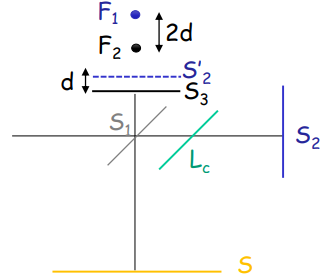
\includegraphics[width=0.3\linewidth]{IM fuochi}
  \caption{Schema dell'apparato rappresentante le due sorgenti virtuali $F_1$ e $F_2$}
\end{figure}


Immaginando che ognuno dei due punti funga da origine di un'onda sferica, possiamo visualizzare i punti nello spazio di uguale luminosità come iperboloidi di rotazione. Se intersechiamo gli iperboloidi con un piano, nel nostro caso rappresentato dallo schermo, dovrebbero essere visualizzati come cerchi concentrici o, nel caso in cui gli specchi non siano ortogonali a causa dell'inclinazione di $S_2$, si visualizzeranno invece delle elissi. 
Se lo specchio $S_2$ non fosse ortogonale e lo specchio $S_3$ venisse spostato in maniera tale che la congiungente tra $F_1$ e $F_2$ sia pressoché parallela allo schermo dovremmo invece visualizzare delle linee parallele verticali. 

\vspace{3mm}

Prendendo un punto sullo schermo possiamo notare che troviamo interferenza costruttiva se la differenza di cammino tra $F_1$ e $F_2$ può essere descritta come:

\begin{equation} 
F_1P - F_2 P = 2d \cos{\theta} = m \lambda 
\end{equation}

Dove la seconda parte è un modo di riscrivere la prima parte in funzione della distanza $d$ tra $F_1$ e $F_2$ e dell'angolo tra la normale allo schermo e $F_1 P$ che chiamiamo $\theta$; la seconda parte indica invece le condizioni di interferenza costruttiva in cui $\lambda$ è la lunghezza d'onda della luce mentre $m \in \mathbb{N}$
determina gli ordini delle fasce luminose.

\vspace{3mm}

Notiamo che per una variazione pari a $\lambda$ della distanza tra i due specchi otteniamo nuovamente delle figure di interferenza nelle stesse posizioni iniziali ma in cui l'n-esimo ordine è sostituito con l'(n-1)-esimo.

\subsection{Misure}
Dalla Equazione (1) possiamo quindi ricavare:

\begin{equation} 
2 n \Delta{x} = N_\lambda \lambda 
\end{equation}

Dove $n$ è l'indice di rifrazione dell'aria, $\Delta{x}$ è lo spostamento di $S_3$ dalla posizione iniziale, $\lambda$ è la lunghezza d'onda del laser e $N_\lambda$ è il numero di frange di interferenza che si vedono passare per un punto dello schermo spostando $S_3$. La presenza del fattore 2 davanti a $\Delta{x}$ tiene conto del fatto che la luce percorre lo spazio $\Delta x$ in ambedue le direzioni.

\vspace{3mm}

Nell'Equazione (2) non conosciamo tuttavia l'indice di rifrazione dell'aria. Per la sua misura utilizzeremo una camera a vuoto. Tenendo conto della differenza di cammino ottico nel caso in cui nella camera vi sia vuoto e nel caso in cui vi sia aria a pressione atmosferica possiamo usare la formula:

\begin{equation}
 2D (n - 1) = N_n \lambda
\end{equation}

In cui $D$ è la lunghezza della cameretta, $n$ è l'indice di rifrazione dell'aria e 1 quello del vuoto, $\lambda$ è la stessa lunghezza d'onda della formula precedente mentre $N_n$ è il numero di righe che passano per un punto dello schermo mentre la cameretta si ripressurizza.

\vspace{3mm}

La lampada a incandescenza non è una sorgente di luce coerente e possiamo quindi notare interferenza solo nel caso in cui i pacchetti di luce provenienti dai due percorsi si incontrano. Possiamo quindi dire che:

\begin{equation} 
L = \Delta{x} 
\end{equation}

dove L è la lunghezza del pacchetto.

Non mettiamo un fattore 2 davanti al termine $\Delta{x}$ come nelle precedenti misure dato che sarebbe necessario un fattore 2 anche davanti al termine $L$.

\vspace{3mm}

L'ultima misura è quella del $\Delta\lambda$ della lampada al sodio. Data la presenza di due frequenze l'effetto che vedremo sarà molto simile a quello di una luce monocromatica ma, a causa della differenza delle due frequenze, spostando $S_3$ noteremo che in alcuni punti le frange luminose di $\lambda_1$ si sovrapporrano con quelle scure di $\lambda_2$, quando ci troveremo in questi punti non saremo in grado di distinguere alcuna frangia di interferenza sullo schermo. Non vedremo frange per:

\begin{equation} 
\Delta_1 = 2 N_1 \frac{\lambda_2}{2} = (2 N_1 + 1) \frac{\lambda_1}{2} 
\end{equation}

E otterremo nuovamente frange per:

\begin{equation} 
\Delta_2 = 2N_2 \lambda_2 =(2 N_1 + 1) \lambda_1 
\end{equation}

Risolvendo per $N_1$ e $N_2$ possiamo quindi giungere alla conclusione che:

\begin{equation} 
\Delta m = m \frac{\lambda_1 \lambda_2}{\lambda_1 {-} \lambda_2} = 2 \Delta{x} 
\end{equation}

Dove consideriamo $m$ il passaggio tra due condizioni di "frangia netta". Ricaviamo quindi che la differenza tra le $\lambda$ della lampada al sodio vale:

\begin{equation} 
\Delta{\lambda} = \frac{m \bar \lambda^2}{2 \Delta{x}} 
\end{equation}

in cui $ \bar \lambda^2$ è la media al quadrato tra i valori delle $\lambda$ della lampada al sodio.




\section{Setup}
Prima di iniziare ci siamo messi in condizione di ortogonalità degli specchi. Abbiamo utilizzato il laser posto su una rotaia allineata con l'apparato e, girando le viti poste sul retro dello specchio $S_2$, abbiamo fatto sovrapporre i due puntini luminosi sullo specchio $S_3$. Abbiamo quindi posto la lente dispersiva sulla rotaia assicurandoci che la luce arrivasse correttamente all'apparato e abbiamo agito nuovamente sulle viti di $S_2$ fino a notare figure di interferenza. Una volta ottenuti dei cerchi concentrici (che confermavano l'ortogonalità tra $S_2$ ed $S_3$) abbiamo aggiustato lo specchio per vedere solo una parte dell'ellisse in maniera tale da semplificare la lettura dei risultati.




\section{Misura $\lambda_{laser}$}
Per effettuare la prima misura abbiamo osservato un punto sullo schermo in cui erano ben visibili fasce scure (possono essere usate anche fasce luminose) e, dopo aver segnato la posizione iniziale letta dal calibro, abbiamo iniziato a girare lentamente la rotella contando le fasce scure che transitavano per il punto. Per diminuire l'incertezza abbiamo dato maggiore importanza alla chiarezza di lettura del calibro piuttosto che ad avere lo stesso tipo di frangia della posizione iniziale.

\vspace{3mm}

Nel nostro caso abbiamo preso 4 set di misure e, con ognuno di essi, abbiamo calcolato $\lambda$ usando l'approssimazione $n = 1$. Abbiamo propagato l'incertezza tramite la formula:

\begin{equation} 
\sigma\lambda= \sqrt{\bigg(\frac{2 n}{N} \sigma_{\Delta X}\bigg)^2 + \bigg({-} \frac{2 n \Delta X}{N^2} \sigma_N\bigg)^2}
\end{equation}

Specifichiamo che abbiamo deciso di utilizzare un incertezza su $N$ pari a 2 dato che riteniamo possibile che l'osservatore abbia confuso una riga precedente con una successiva durante il conto di quasi 200 righe.
Una volta ottenuti questi risultati abbiamo utilizzato una media pesata ed abbiamo ottenuto:
\[ \lambda_{laser} = 0,617 \pm 0,016 \; \mu m \]
Riportiamo quindi in Tabella 1 i dati grezzi ed i risultati parziali.


%tabella lambda
\begin{table}[h!]
\centering
\begin{tabular}{ | c | c | c | c | c | c | c | c |}
\hline
 \# & $X_1 \; [m \cdot 10^{-5}/5]$ & $X_2 \; [m \cdot 10^{-5}/5]$ & $\Delta X \; [m \cdot 10^{-5}/5]$ & $\Delta X \; [\mu m]$ & $N_\lambda$ & $\lambda \; [\mu m]$ & $\sigma\lambda \; [\mu m]$\\
\hline
   1 & 100 & 131 & 31 & 62 & 200 & 0,620 & 0,029\\
   2 & 150 & 178 & 28 & 56 & 177 & 0,633 & 0,033\\
   3 & 200 & 231 & 31 & 62 & 196 & 0,633 & 0,030\\
   4 & 250 & 275 & 25 & 50 & 171 & 0,585 & 0,034\\
\hline
\end{tabular}
\caption{Dati calcolo $\lambda$}
\label{table:1}
\end{table}

%immagine risultato laser
\begin{figure}[h!]
  \centering
  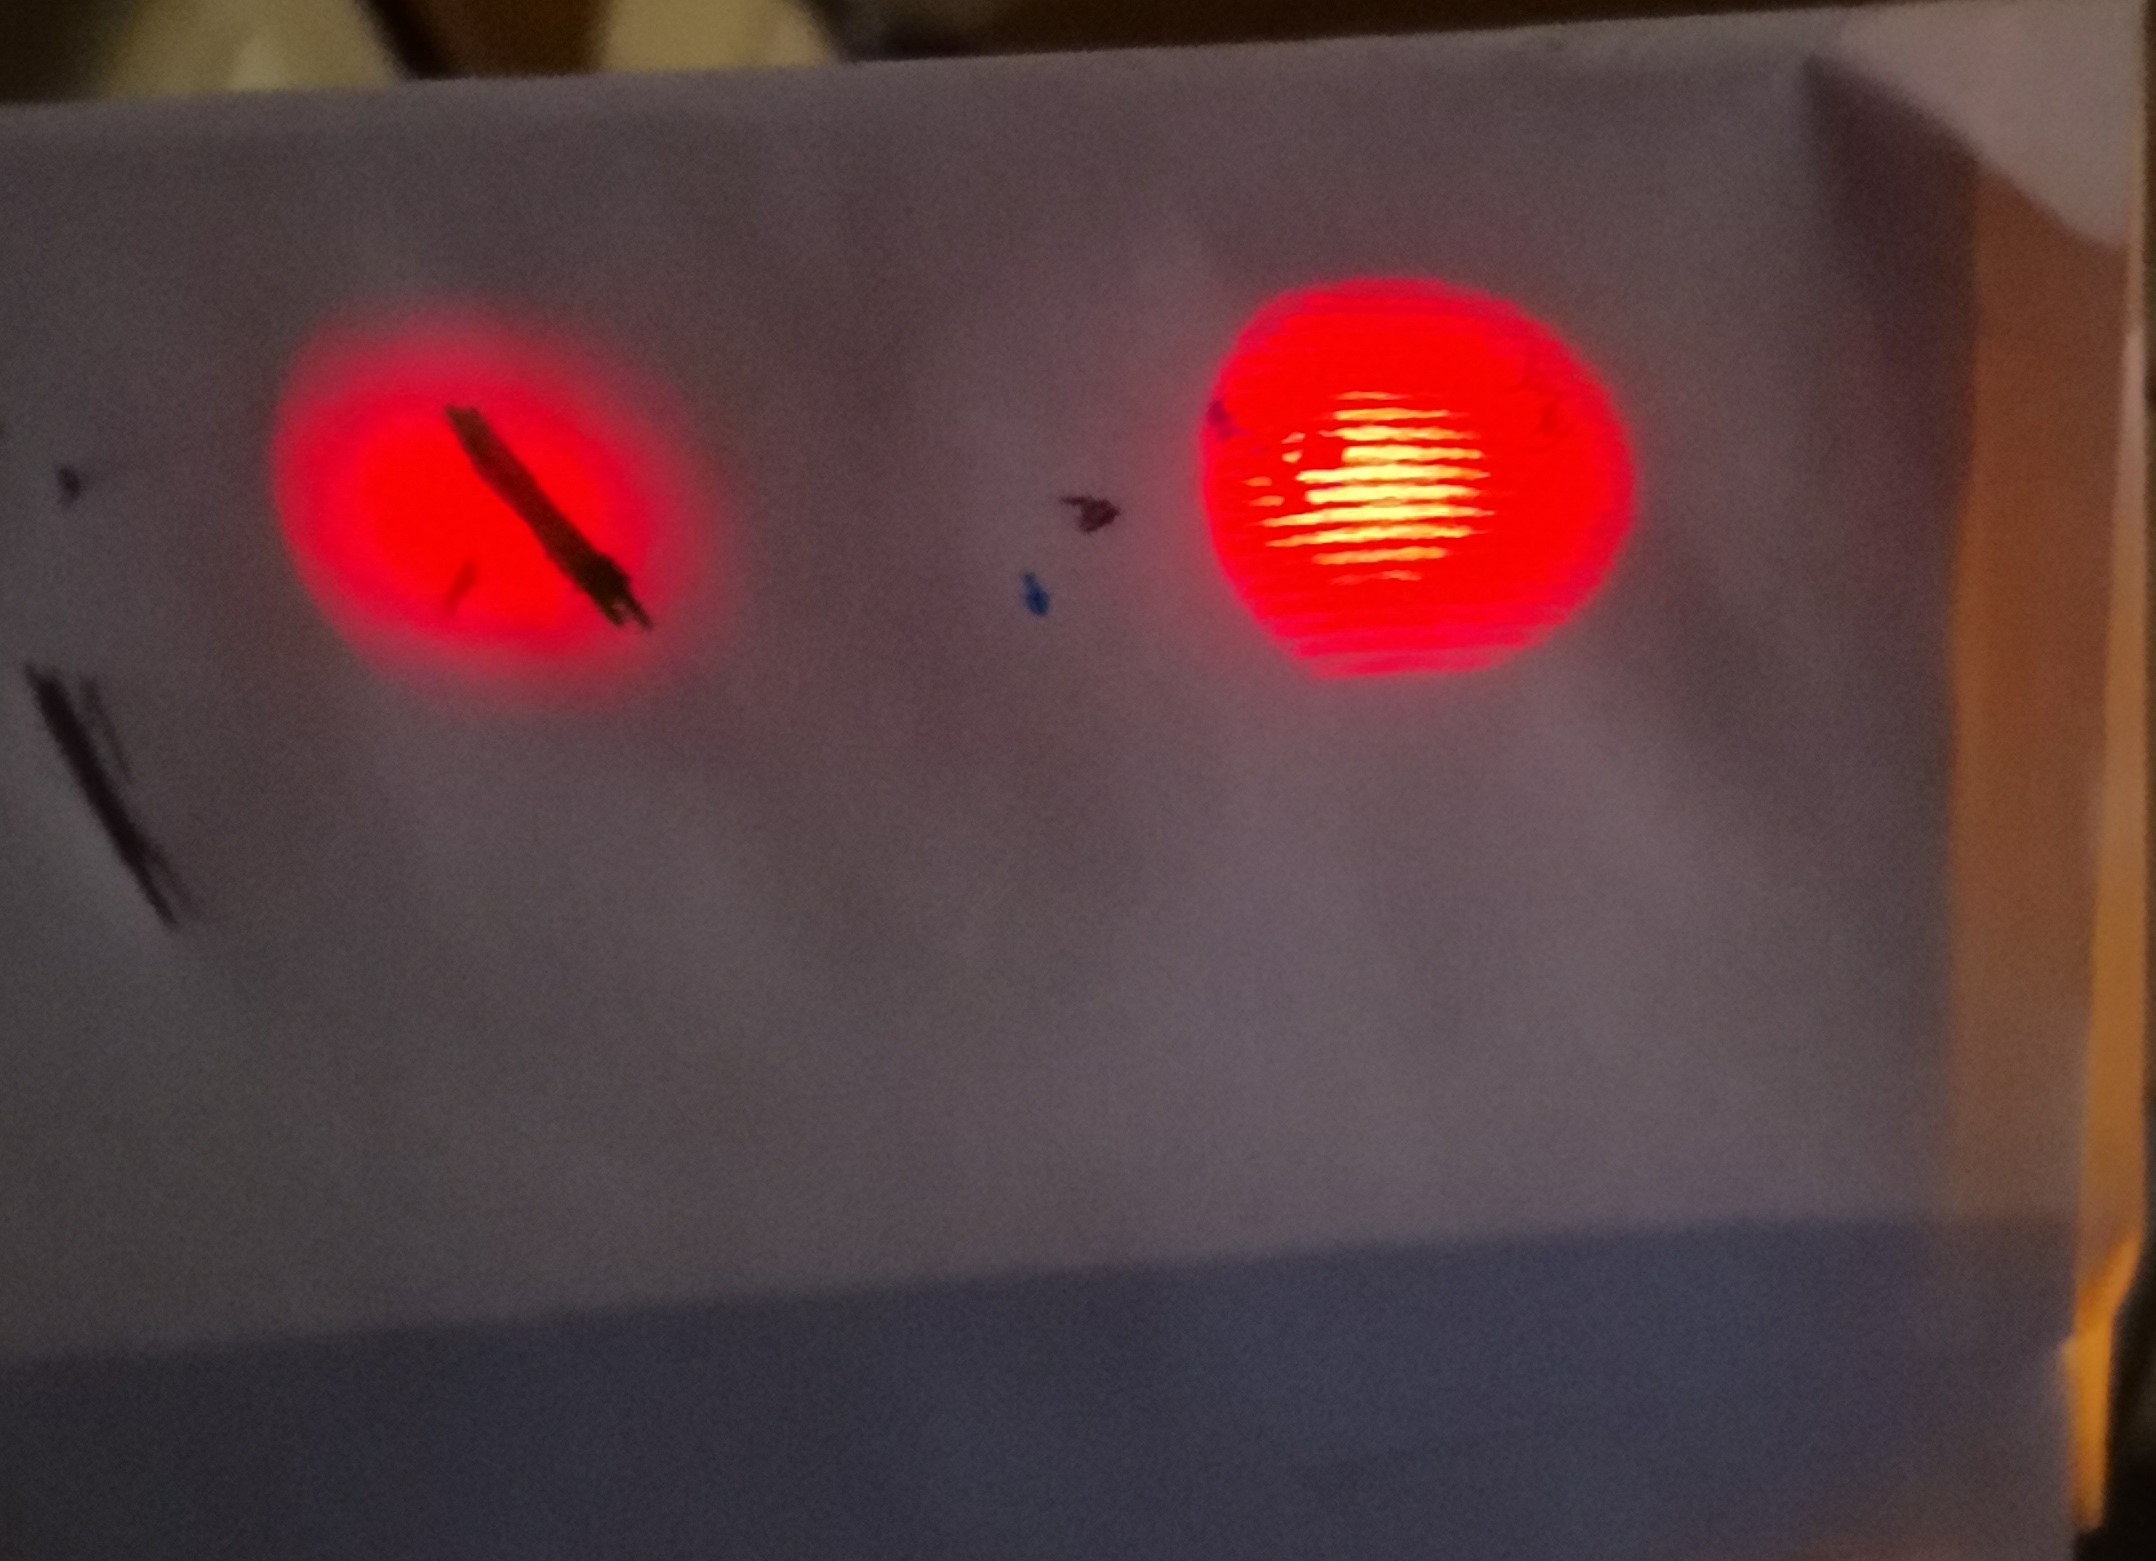
\includegraphics[width=0.6\linewidth]{IM laser}
  \caption{Foto dell'interferenza del laser}
\end{figure}

%immagine etichetta
\begin{figure}[h!]
  \centering
  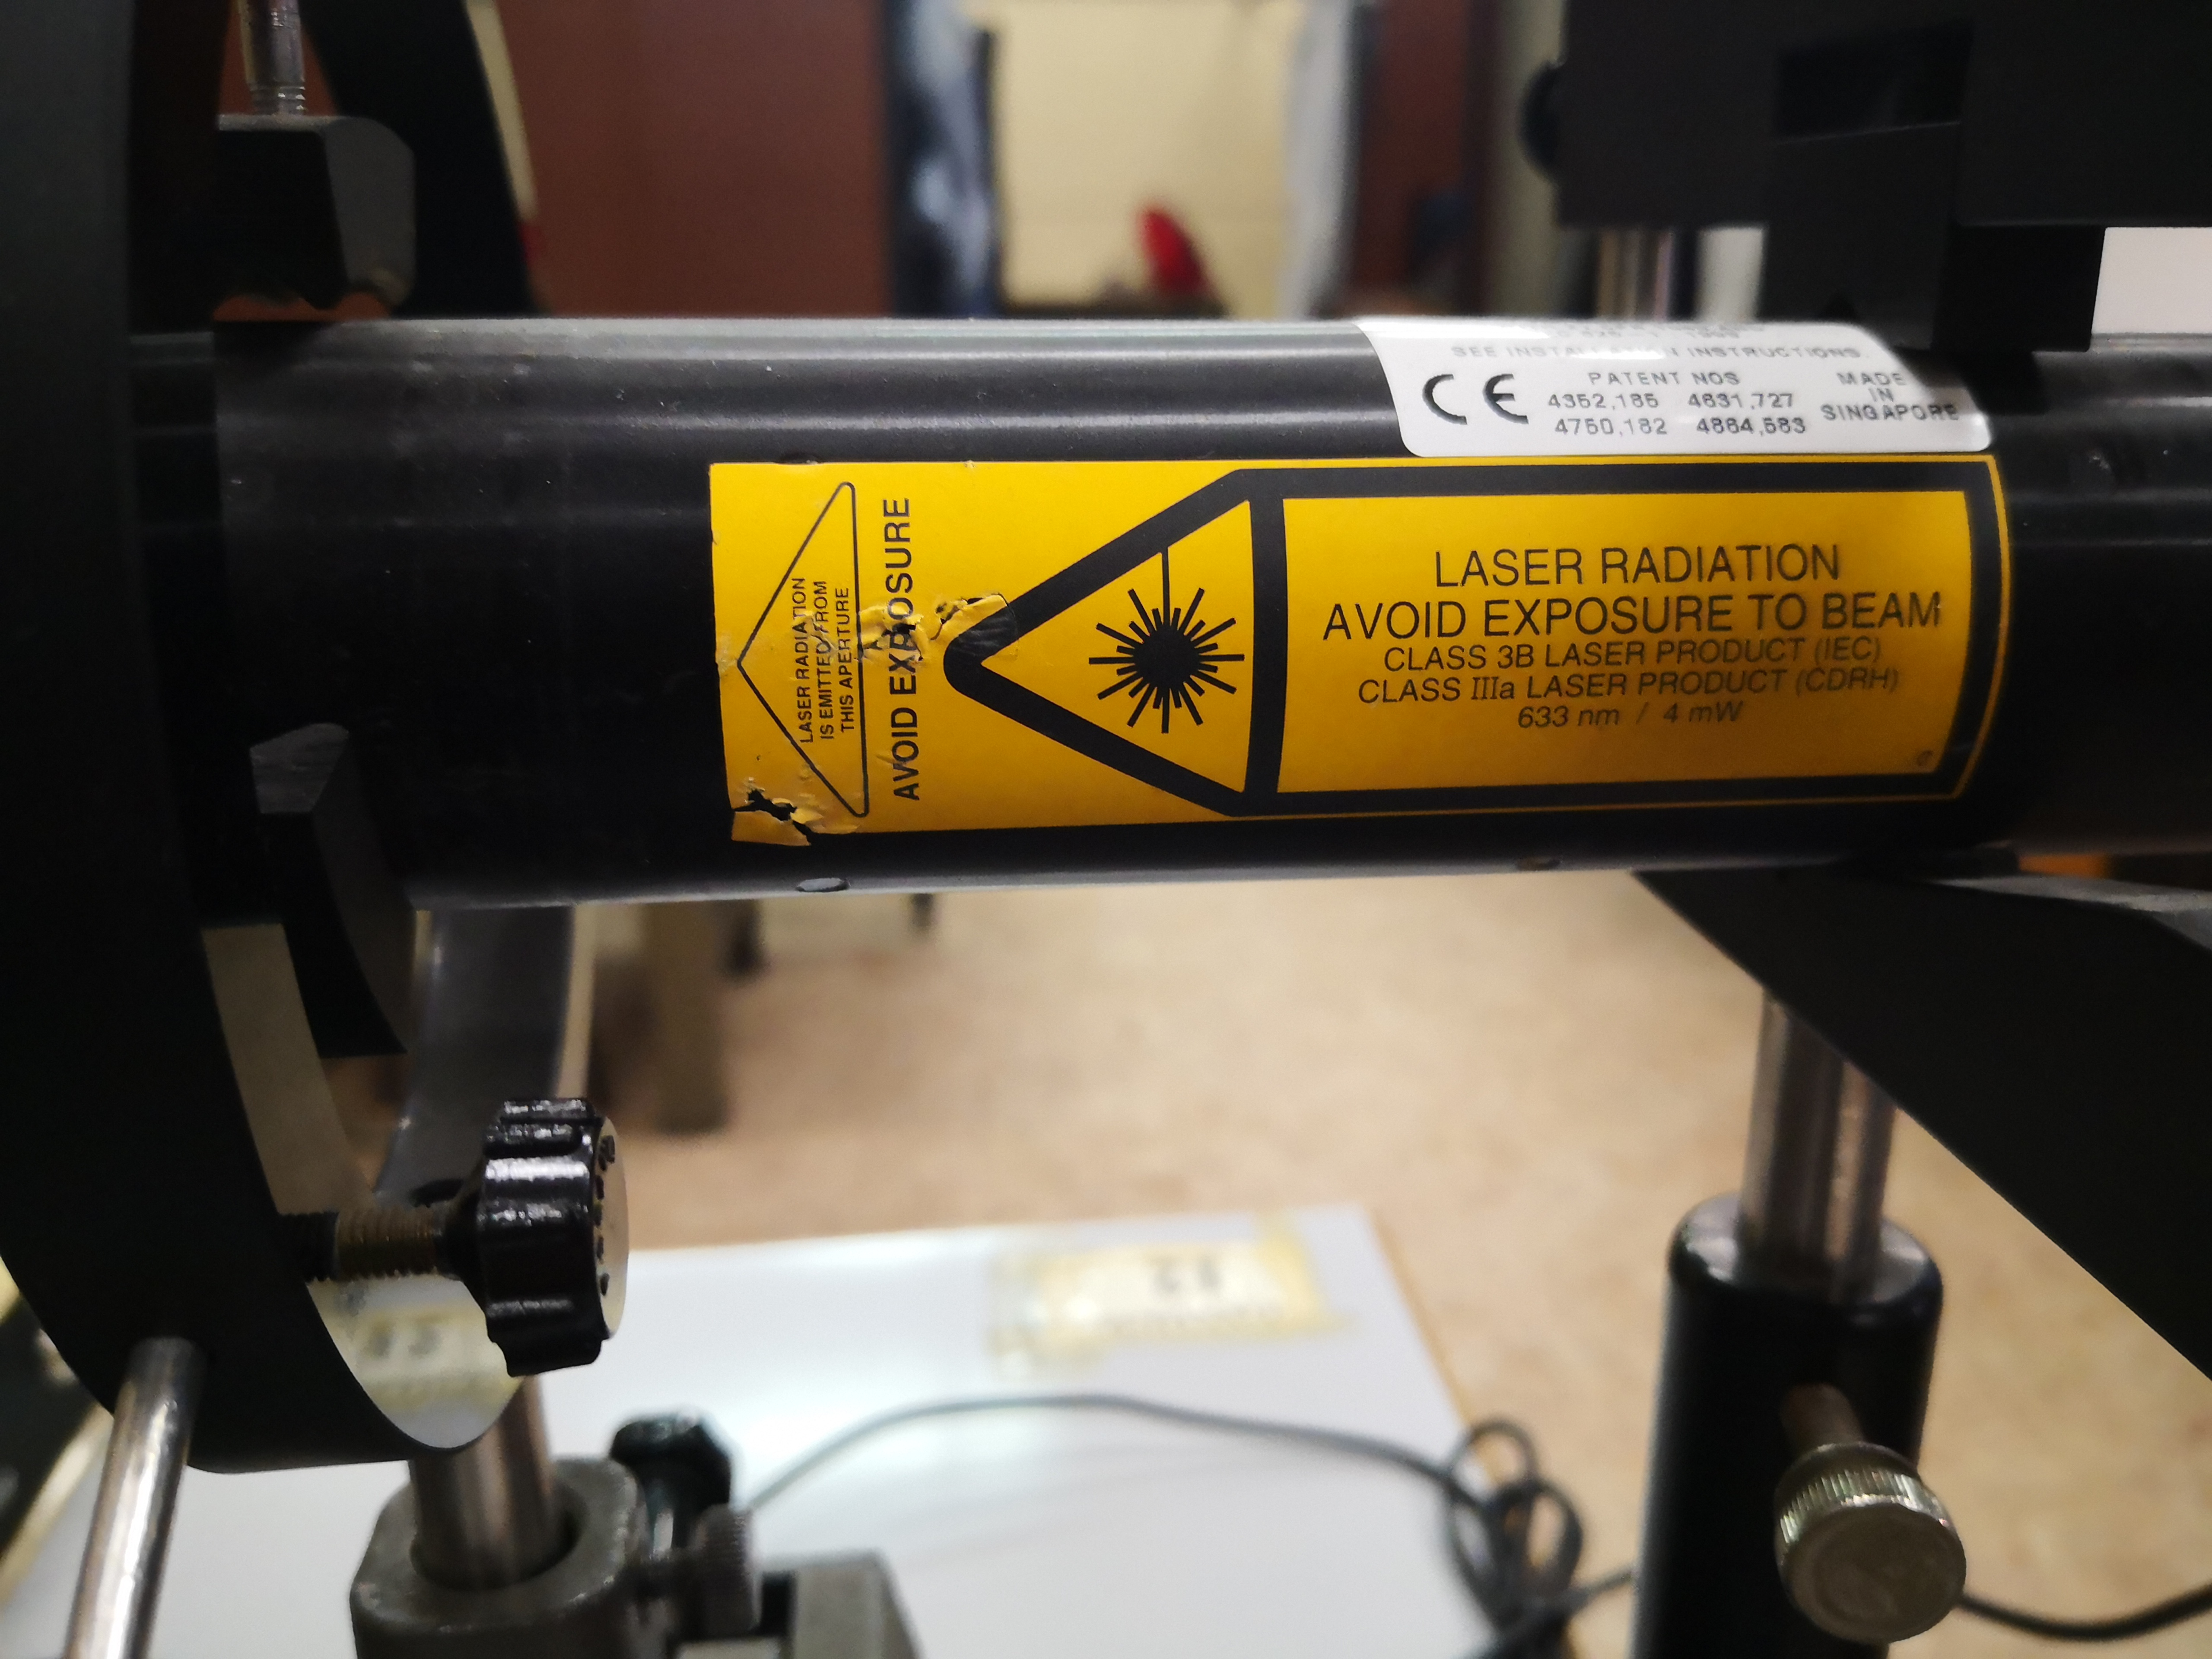
\includegraphics[width=0.6\linewidth]{IM etichetta laser}
  \caption{Etichetta con informazioni del laser}
\end{figure}

\pagebreak

\section{Misura indice di rifrazione dell'aria}
Per effettuare la seconda misura abbiamo posizionato la camera a vuoto tra $S_1$ e $S_3$. Ci siamo accertati che la valvola di ingresso dell'aria fosse chiusa e abbiamo acceso la pompa a vuoto fino a quando la pressione si è stabilizzata (abbiamo osservato il manometro). Per effettuare la misura abbiamo aperto leggermente la valvola contando le frange che transitavano per un punto dello schermo da noi scelto (in maniera analoga alla misura di $\lambda_{laser}$).

%immagine etichetta
\begin{figure}[h!]
  \centering
  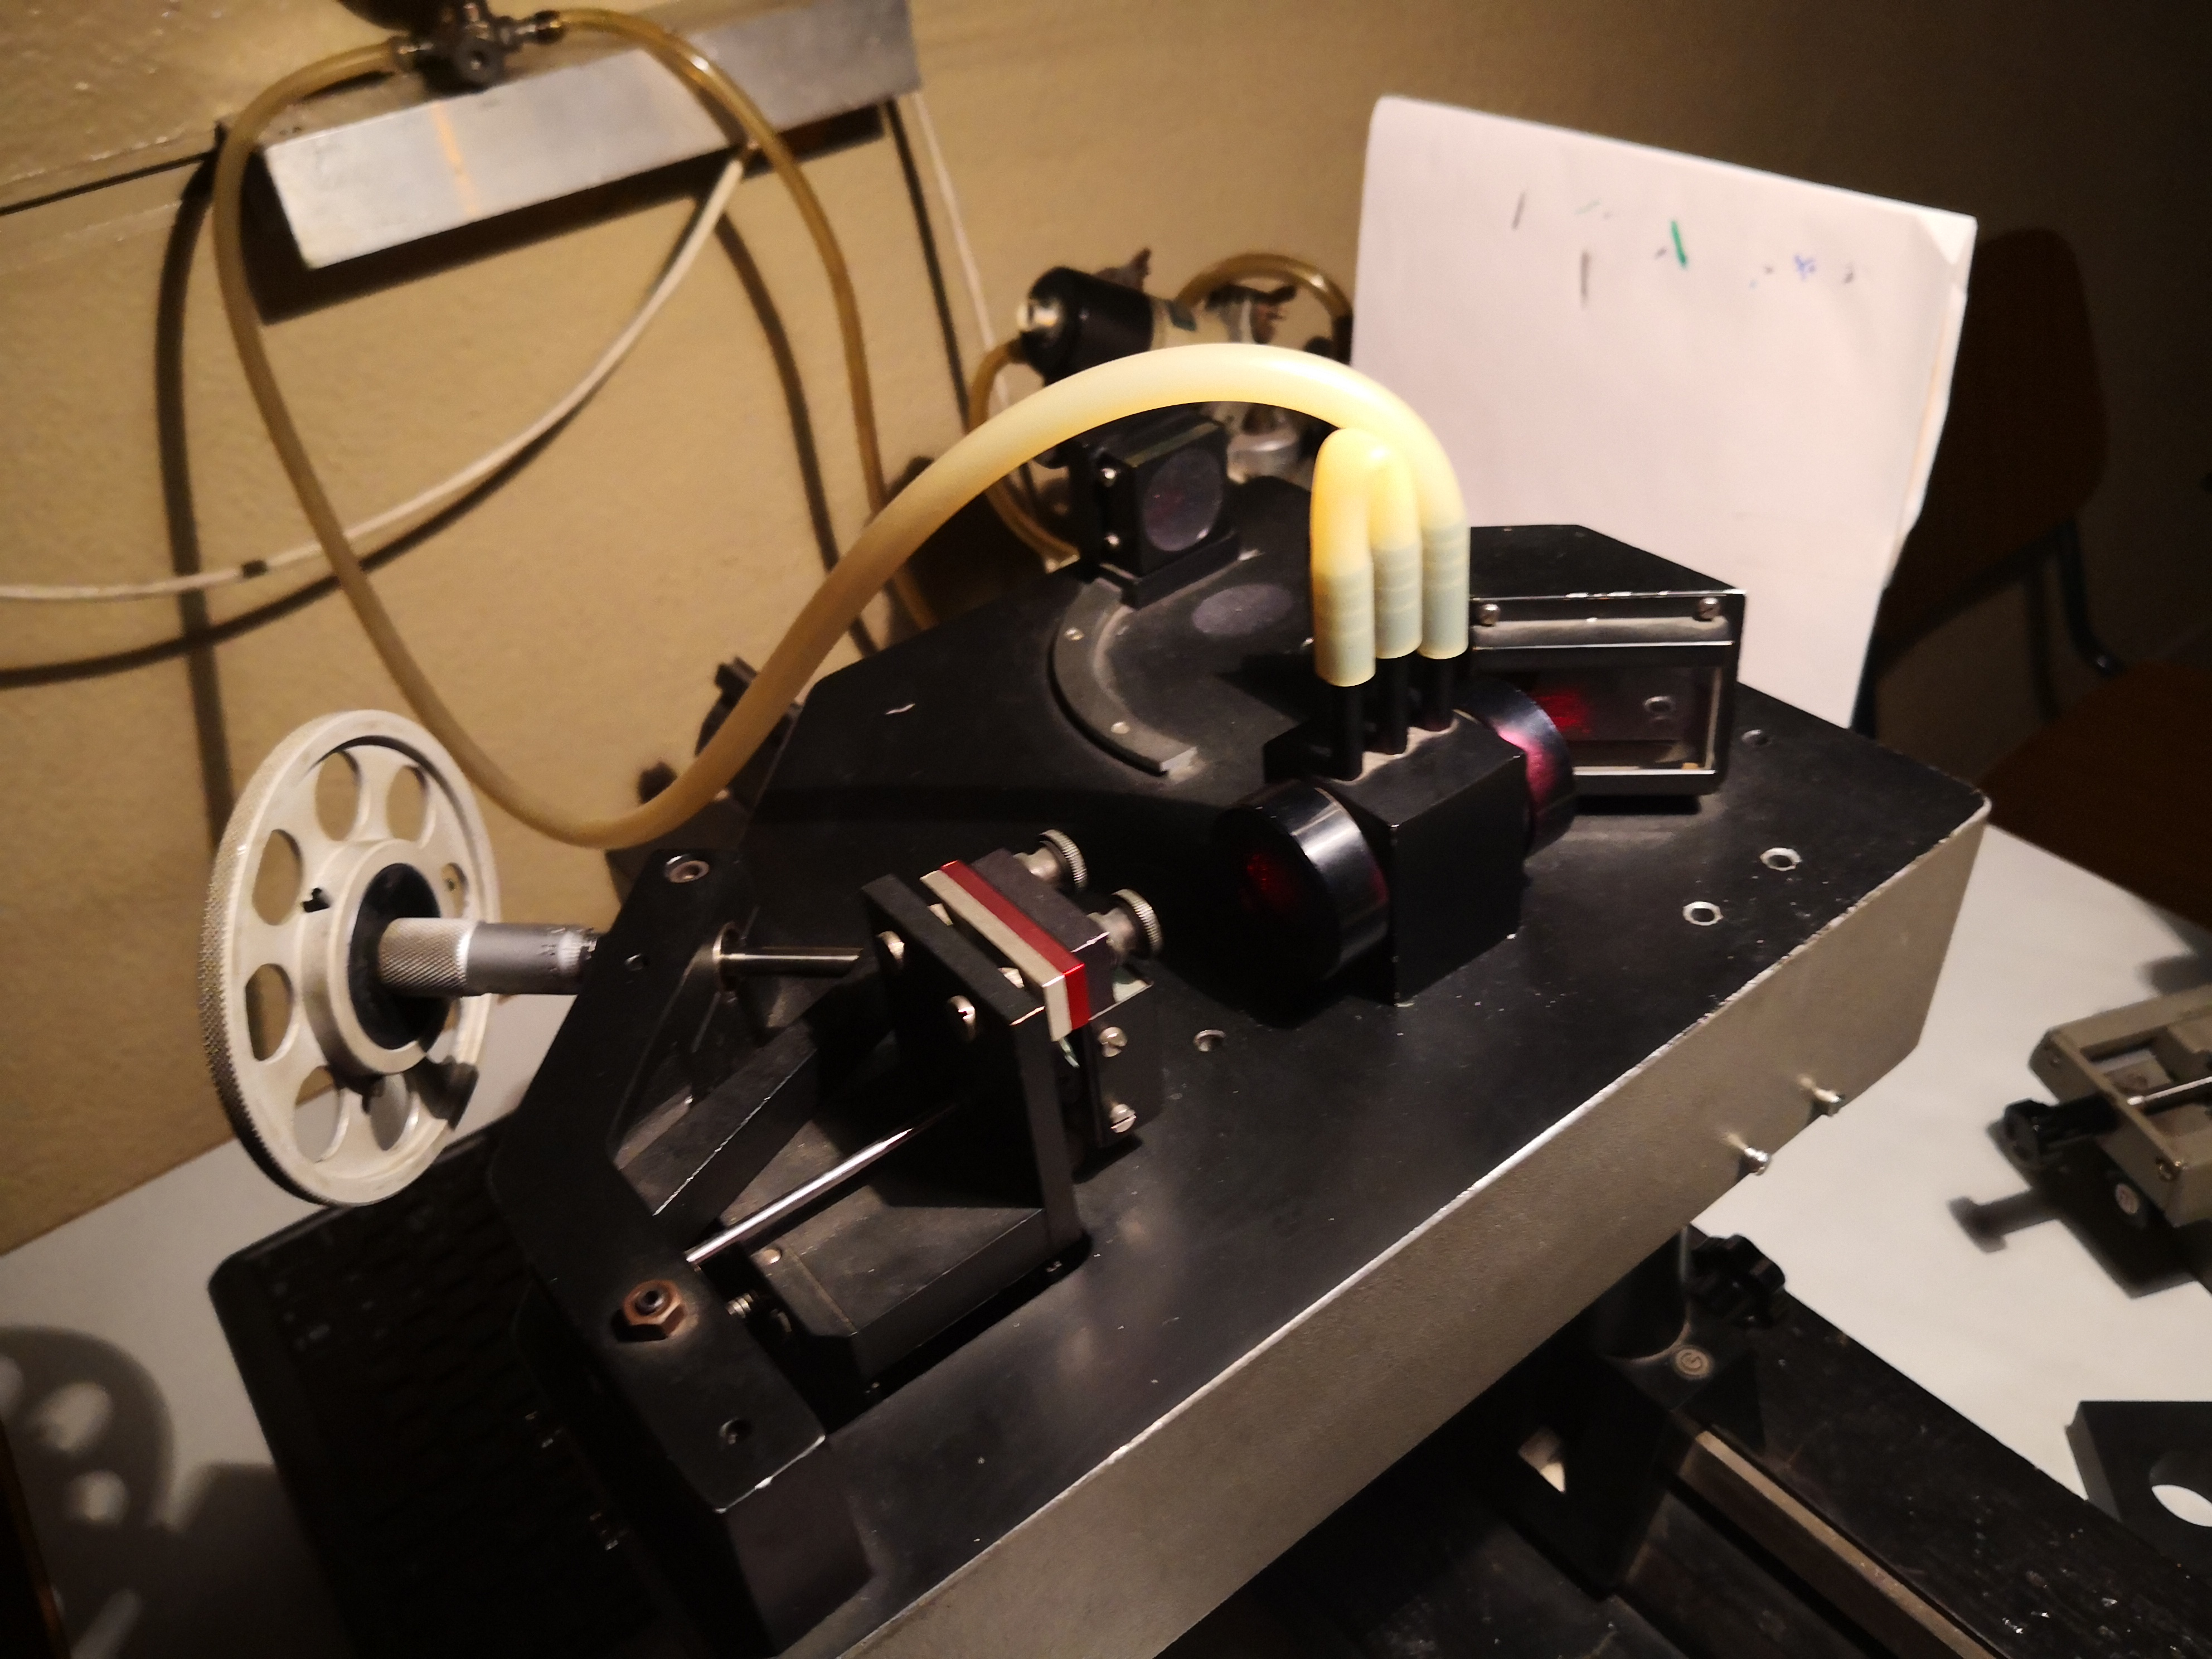
\includegraphics[width=0.6\linewidth]{IM cameretta}
  \caption{Immagine della camera a vuoto attaccata alla pompa tramite il tubo giallo}
\end{figure}

\pagebreak

Per l'analisi dati abbiamo utilizzato lo stesso metodo utilizzato in Misura 1 dove tuttavia l'incertezza è stata calcolata tramite la propagazione degli errori con le incertezze di $\lambda$, $D$ ed $N$, tramite la formula

\begin{equation}
\sigma_n = \sqrt{ \bigg(\frac{N}{2D} \sigma_\lambda \bigg)^2 + \bigg({-} \frac{N \lambda}{2 D^2} \sigma_D \bigg)^2 + \bigg(\frac{\lambda}{2D} \sigma_N \bigg)^2} 
\end{equation}

utilizzando la $\lambda$ calcolata in Misura 1. Abbiamo ottenuto il seguente valore:
\[ n_{aria} = 1,000254 \pm 7 \cdot 10^{-6} \]

Data la mancanza della conoscenza di fattori quali la temperatura della stanza e un'accurata misurazione della pressione atmosferica, riportiamo il valore dell'indice di rifrazione dell'aria in condizioni standard reperito dal sito \textit{https://it.wikipedia.org/wiki/Indice\_di\_rifrazione}.
\[ n_{aria} = 1,000293  \]
Riteniamo plausibile il valore ottenuto, sebbene disti diverse deviazioni standard dal valore teorico. Il discostamento potrebbe essere causato dalla misura del valore teorico effettuata in diverse condizioni di temperatura e pressione.

Riportiamo in Tabella 2 i dati grezzi ed i risultati parziali


%tabella n
\begin{table}[h!]
\centering
\begin{tabular}{ | c | c | c | c | }
\hline
 \# & $N_n$ & $n$ & $\sigma_n$\\
\hline
   1 & 40 & 1,000247 & $1,5 \cdot 10^{-5}$\\
   2 & 41 & 1,000253 & $1,5 \cdot 10^{-5}$\\
   3 & 42 & 1,000259 & $1,5 \cdot 10^{-5}$\\
   4 & 42 & 1,000259 & $1,5 \cdot 10^{-5}$\\
\hline
\end{tabular}
\caption{Dati calcolo indice di rifrazione aria}
\label{table:2}
\end{table}




\section{Sistema $\lambda$-$n$}
I dati forniti in Misura 1 e Misura 2 sono fortemente influenzati dall'iniziale assunzione di porre $n = 1$ in Misura 1. Per correggere questo errore abbiamo applicato due metodi, non essendo in grado di identificare il migliore prima di effettuare i calcoli. 



\subsection{Sistema}
Per il primo metodo abbiamo messo a sistema le equazioni (2) e (3) ottenendo quindi:

\begin{equation} 
n= \frac{1}{1 - \frac{\Delta_x}{N_\lambda} \frac{N_n}{D}} 
\end{equation}

In cui abbiamo raccolto le misure

\[ a = \frac{\Delta_x}{N_\lambda} \]
\[ b = \frac{N_n}{D} \]

Per poter eseguire l'analisi statistica dato che non avremmo potuto ricavare misure singole dai dati, al contrario di quanto fatto per misure 1 e 2 provenendo essi sia dalla misura per $\lambda$ che dalla misura per $n$. Abbiamo calcolato lincertezza sia per $a$ che per $b$ tramite la formula di propagazione degli errori e, dai valori risultati, abbiamo calcolato una media pesata ottenendo i valori di $a$, $\sigma_a$, $b$ e $\sigma_b$ utilizzati per calcolare $n$ e, tramite la propagazione degli errori, $\sigma_n$. il valore risultato è:
\[ n_{aria} = 1,000256 \pm 1,4 \cdot 10^{-5} \]
Da cui abbiamo proceduto a eseguire in maniera analoga alla Misura 1, il calcolo di $\lambda$ in cui l'errore, per tenere conto dell'incertezza su n, è calcolato come:

\begin{equation} 
\sigma\lambda= \sqrt{\left(\frac{2 n}{N_\lambda} \sigma_{\Delta x}\right)^2 + \left(\frac{2 \Delta x}{N_\lambda} \sigma_n\right) + \left({-} \frac{2 n \Delta x}{N_\lambda^2} \sigma_{N_\lambda}\right)^2} 
\end{equation}

Abbiamo quindi ottenuto il valore:
\[ \lambda_{laser} = 0,619 \pm 0,016 \; \mu m \]
Per controllare la tabella con i risultati parziali controllare in Appendice Grafici e tabelle immagine %numero immagine



\subsection{Metodo ricorsivo}
Per il secondo metodo abbiamo eseguito gli stessi calcoli delle Misure 1 e 2. Inizialmente abbiamo supposto $n = 1$ e da esso abbiamo calcolato $\lambda_1$ e $n_1$ ottenendo gli stessi risultati sopraindicati, abbiamo poi utilizzato il nuovo valore di $n$ ottenuto per calcolare nuovamente sia $\lambda_2$ che $n_2$. dopo aver iterato il processo 4 volte abbiamo ottenuto dei risultati che non variavano in maniera significativa, riportiamo la differenza dei valori tra la terza e la quarta iterazione:
\[ \lambda_{laser} = 1,029 \cdot 2^{-11} \pm 2,6 \cdot 2^{-13} \; \mu m \]
\[ n_{aria} = 1,663 \cdot 10^{-11} \pm 0 \]
Sebbene alla terza iterazione non notassimo differenze nelle cifre significative da noi utilizzate, abbiamo deciso di procedere comunque a una quarta dato per annullare completamente la differenza di $\sigma_n$. 

\vspace{3mm}

Riportiamo quindi i valori trovati:
\[ \lambda_{laser} = 0,619 \pm 0,016 \; \mu m \]
\[ n_{aria} = 1,000255 \pm 2 \cdot 10^{-6} \]

I risultati delle singole ricorsioni sono riportati in Tabella 6 in Appendice.



\subsection{Analisi risultati}
Riportiamo in Figura 7 e 8 i grafici per l'analisi dei risultati.

%grafici lambda e n
\begin{figure}[h!]
  \centering
  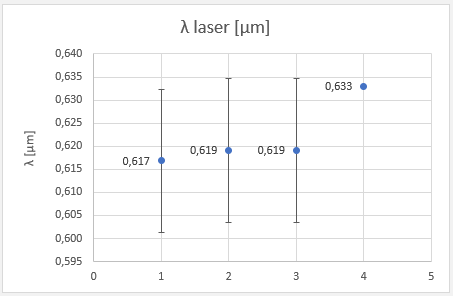
\includegraphics[width=0.6\linewidth]{IM grafico risultati lambda}
  \caption{Comparazione risultati $\lambda_{laser}$}
\end{figure}

\begin{figure}[h!]
  \centering
  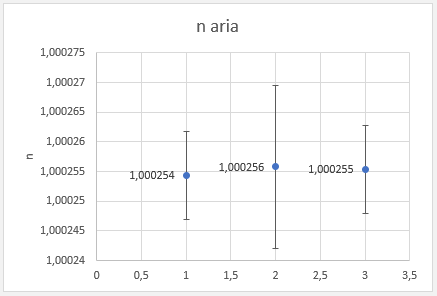
\includegraphics[width=0.6\linewidth]{IM grafico risultati n}
  \caption{Comparazione risultati indice di rifrazione dell'aria}
\end{figure}


Riteniamo che i nostri risultati per quanto riguarda $\lambda$ possano essere considerati attendibili dato che si trovano tutte entro una deviazione standard di distanza dal valore vero fornito dal costruttore del laser di $0,633 \; \mu m$. Dato che i due metodi producono il medesimo valore di $\lambda$, non avendo un valore di riferimento accurato per $n$, li riteniamo entrambi validi e non siamo in grado di definire il migliore.



\section{Misura lunghezza pacchetto di luce bianca}

\subsection{Setup}
In seguito alle misure con laser siamo quindi passati alla misura della lunghezza del pacchetto d'onda della luce bianca. Dato che la lunghezza di coerenza della luce bianca è molto più piccola rispetto a quella del laser, ci siamo dovuti porre in condizione in cui l'asse tra i due fuochi e lo specchio fossero pressoché paralleli, al fine di ottenere interferenza. Per trovare questa condizione abbiamo iniziato a girare la rotella fino ad avere una figura di interferenza composta da linee verticali leggermente curve. Abbiamo quindi continuato fino a quando la curvatura ha cambiato direzione e ci siamo posizionati nel punto in cui notavamo il cambio di curvatura. Abbiamo quindi spento il laser e abbiamo posizionato la fibra ottica sulla rotaia direttamente davanti a $S_1$ (la lente divergente è necessaria solo per il laser). Nonostante il posizionamento eseguito con il laser non abbiamo notato interferenza e abbiamo quindi continuato a girare la rotella finché sullo schermo abbiamo iniziato a vedere un'alternanza di varie frange colorate come in Figura 9.

%immagine pacchetto di luce
\begin{figure}[h!]
  \centering
  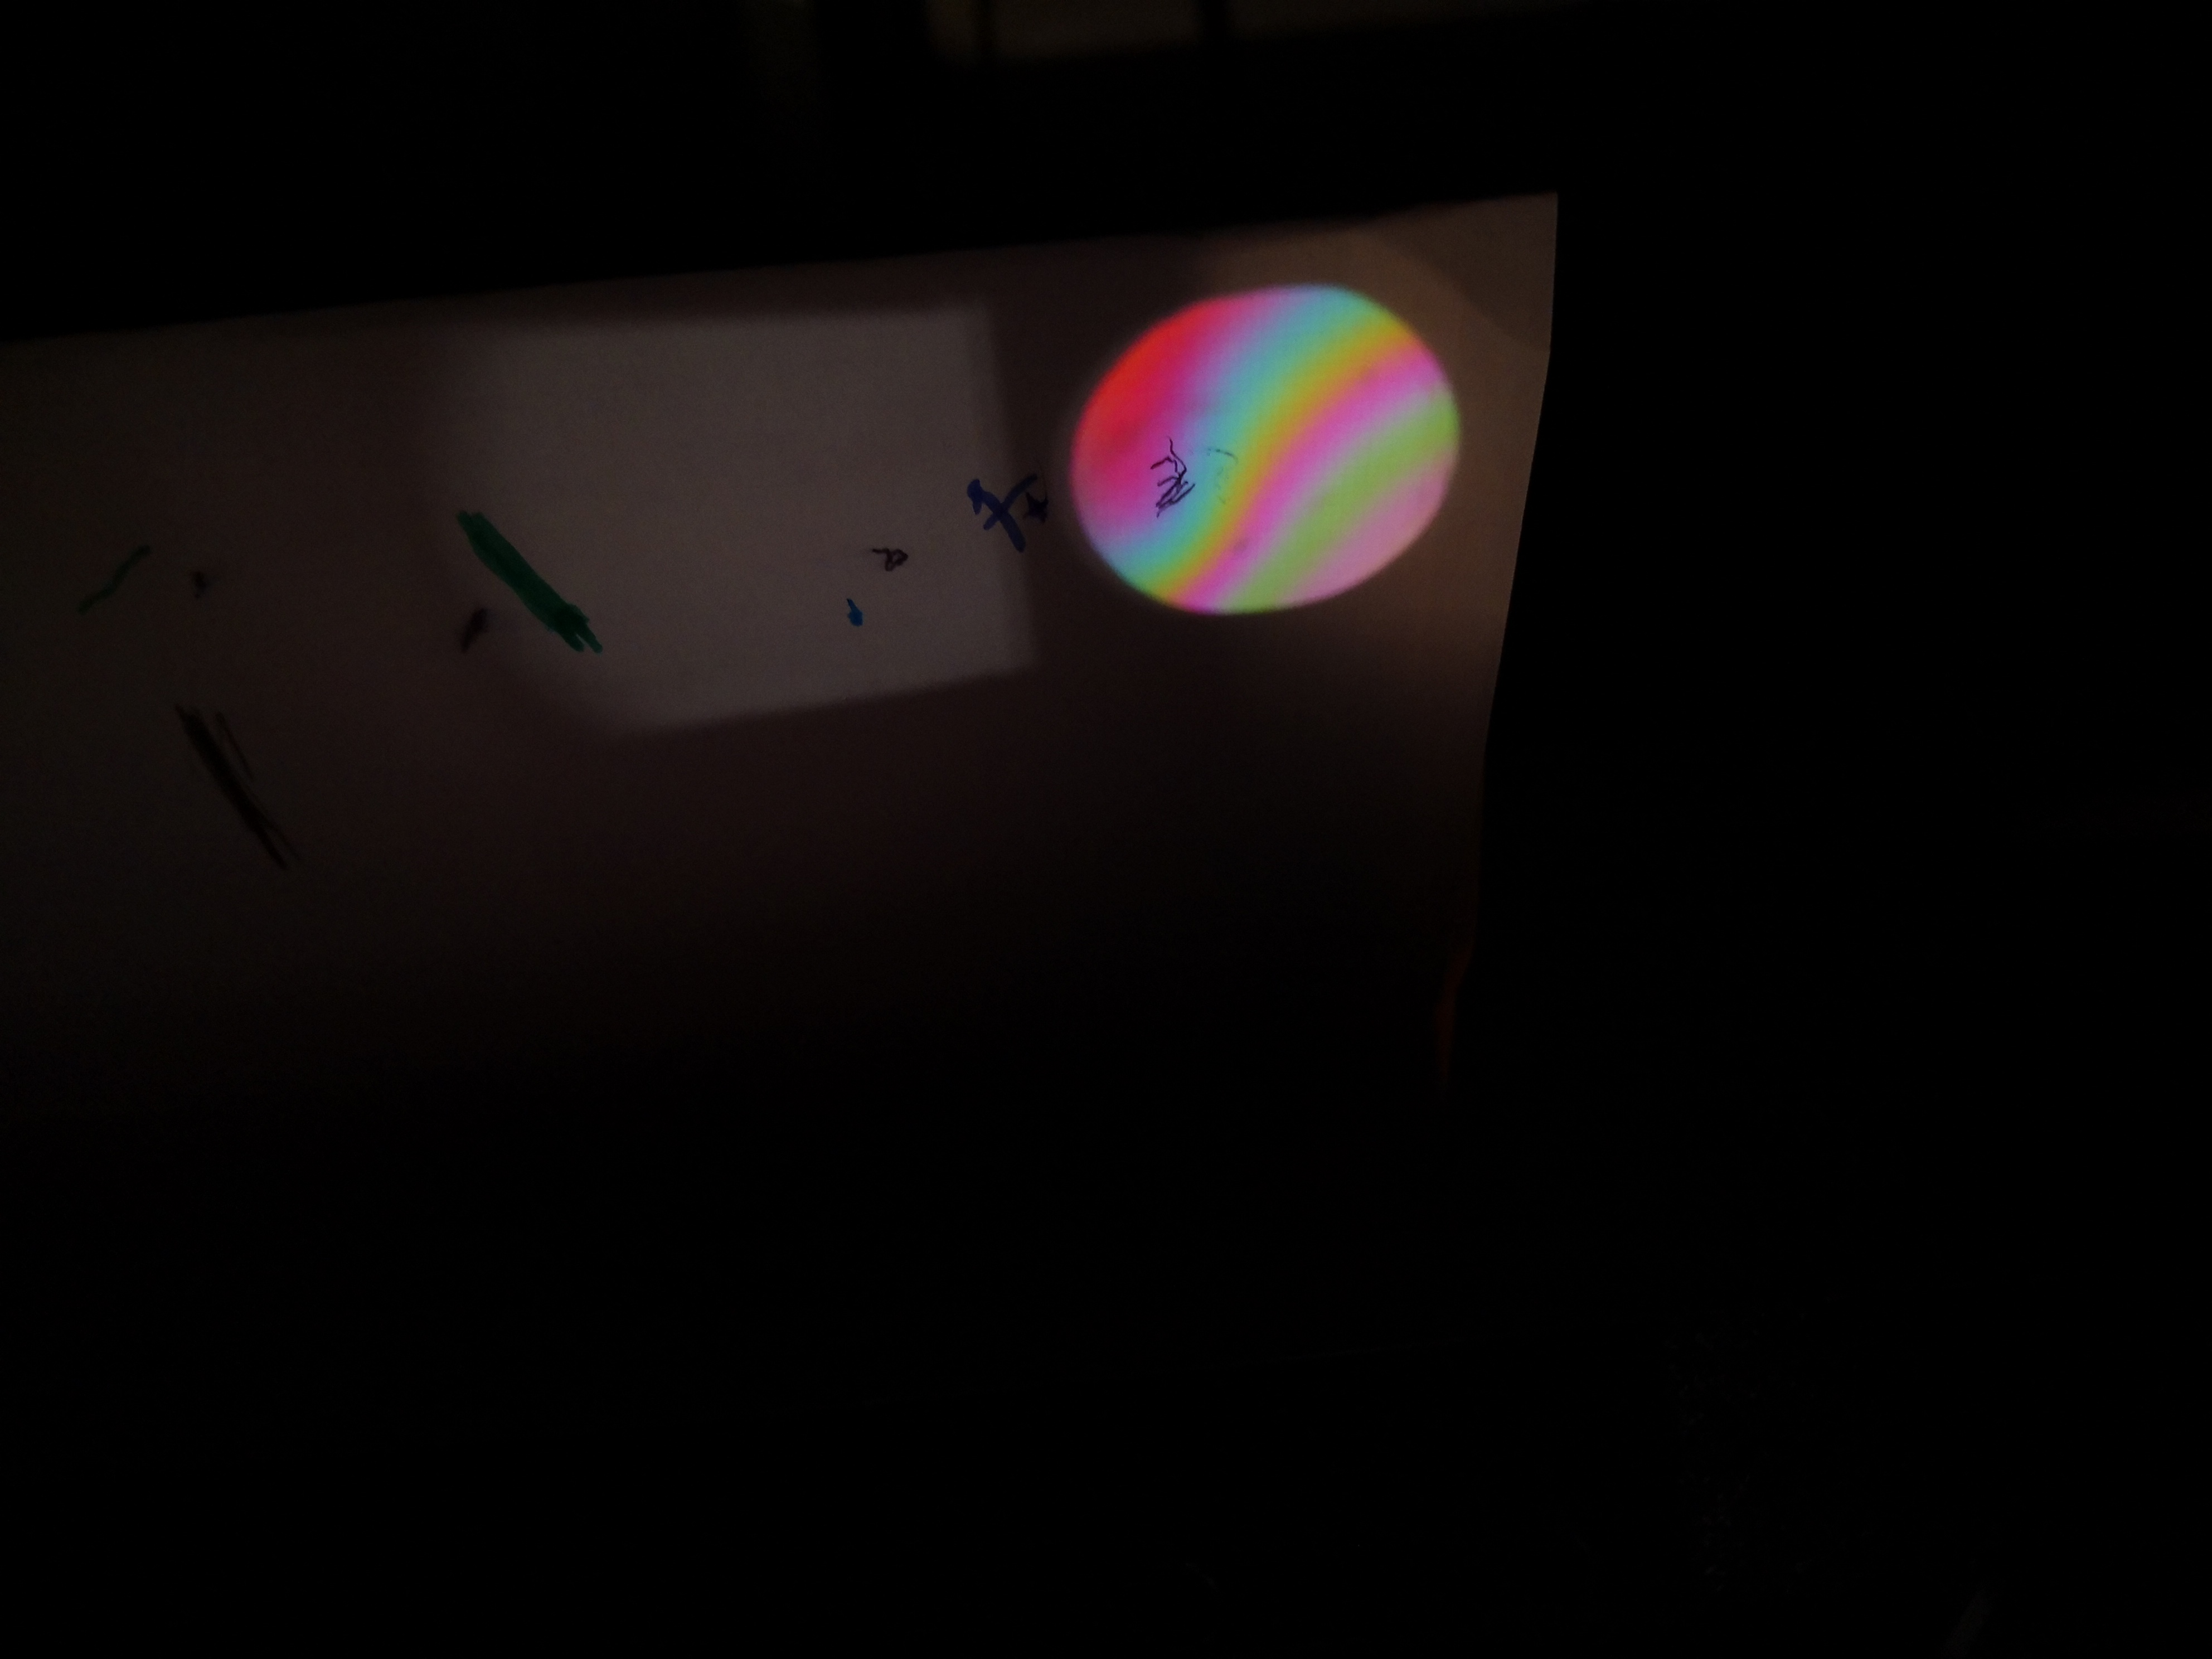
\includegraphics[width=0.6\linewidth]{IM pacchetto}
  \caption{Interferenza del pacchetto di luce bianca}
\end{figure}


\subsection{Misura}
Ci siamo posti in una condizione in cui non riuscivamo a vedere frange, abbiamo iniziato a girare la rotella fino a iniziare a vedere le frange e abbiamo segnato la posizione. Abbiamo poi continuato a girare la rotella fino a tornare in condizione in cui lo schermo era completamente bianco segnando il punto in cui non riuscivamo più a vedere le frange.

\vspace{3mm}

Abbiamo effettuato un totale di 4 misure, girando la rotella sia in senso orario che in senso antiorario per ridurre possibili errori. Dai nostri dati abbiamo ottenuto, usando una media aritmetica, un valore del pacchetto pari a:
\[ L_{pacchetto} = 7,5 \pm 2,8 \; \mu m \]
Notiamo che la misura ha un valore dello stesso ordine di grandezza dell'incertezza strumentale, usato come incertezza, e riteniamo quindi che possa essere errata. Purtroppo non abbiamo un valore preciso con cui compararla. Dopo con un confronto con il gruppo Ve-13, che ha ottenuto un valore di $L_{pacchetto}=14 \; \mu m$ riteniamo che la misura abbia un'ordine di grandezza coerente anche se, avendo usato lampade diverse, non possiamo considerarlo un valore adatto a una comparazione che vada oltre l'ordine di grandezza.

\vspace{3mm}

Riportiamo in Tabella 3 i dati grezzi e i risultati parziali.


%tabella pachetto d'onda luce bianca
\begin{table}[h!]
\centering
\begin{tabular}{ | c | c | c | c | c | }
\hline
\# & $X_1 \; [m \cdot 10^{-5}/5]$ & $X_2 \; [m \cdot 10^{-5}/5]$ & $\Delta X \; [m \cdot 10^{-5}/5]$ & $\Delta \; [\mu m]$\\
\hline
   1 & 1591 & 1587 & 4 & 8\\
   2 & 1587 & 1591 & 4 & 8\\
   3 & 1587 & 1590 & 3 & 6\\
   4 & 1591 & 1587 & 4 & 8\\
\hline
\end{tabular}
\caption{Dati calcolo pacchetto di luce bianca}
\label{table:3}
\end{table}


Abbiamo provato a mettere un filtro verde davanti alla luce per provare a vedere cosa succedesse nel caso di una luce più simile a una luce monocromatica. Dopo avere raccolto una sola misura (per avere un termine di paragone quantitativo) abbiamo ricavato una lunghezza del pacchetto pari a $68 \; \mu m$. Come previsto la presenza del filtro verde aumenta la lunghezza di coerenza.



\section{Misura $\Delta\lambda$ della lampada al sodio}
Per la quarta abbiamo disconnesso la fibra ottica dalla lampada ad incandescenza e l'abbiamo attaccata alla lampada Na. Una volta attaccata la lampada abbiamo iniziato a vedere delle frange gialle in maniera simile a quanto visto con il laser. Abbiamo ruotato la rotella fino a vedere le frange scure scomparire e segnato quindi la prima misura, usata come riferimento anche per le altre. Abbiamo continuato a girare la rotella vedendo le frange scure ricomparire e, dopo aver continuato a ruotare, siamo tornati nella condizione in cui le frange scure scomparivano. Abbiamo ripetuto i passaggi per quatro volte, prendendo le posizioni in cui le frange scomparivano, ma avendo colpito accidentalmente l'apparato abbiamo dovuto fermarci e rieseguire la messa a punto dell'apparato prima di prendere altre 5 misure.

\vspace{3mm}

\clearpage

Riportiamo in Tabella 4 e 5 i dati grezzi e i risultati parziali

%tabella Na 1
\begin{table}[h!]
\centering
\begin{tabular}{ | c | c | c | c | c | c | c | c |}
\hline
 \# & $X_1 \; [m \cdot 10^{-5}/5]$ & $X_2 \; [m \cdot 10^{-5}/5]$ & $\Delta X \; [m \cdot 10^{-5}/5]$ & $\Delta X \; [\mu m]$ & $M$ & $\Delta\lambda \; [\textrm{Å}]$ & $\sigma_{\Delta\lambda} \; [\textrm{Å}]$\\
\hline
   1 & 1583 & 1495 & 88 & 176 & 1 & 9,866 & 0,159\\
   2 & 1583 & 1293 & 290 & 580 & 2 & 5,987 & 0,029\\
   3 & 1583 & 1139 & 444 & 888 & 3 & 5,866 & 0,019\\
   4 & 1583 & 1092 & 491 & 982 & 4 & 7,073 & 0,020\\
\hline
\end{tabular}
\caption{Dati calcolo $\Delta\lambda_{Na}$ 1}
\label{table:4}
\end{table}


%tabella Na 2
\begin{table}[h!]
\centering
\begin{tabular}{ | c | c | c | c | c | c | c | c |}
\hline
\# & $X_1 \; [m \cdot 10^{-5}/5]$ & $X_2 \; [m \cdot 10^{-5}/5]$ & $\Delta X \; [m \cdot 10^{-5}/5]$ & $\Delta X \; [\mu m]$ & $M$ & $\Delta\lambda \; [\textrm{Å}]$ & $\sigma_{\Delta\lambda} \; [\textrm{Å}]$\\
\hline
   1 & 1580 & 1430 & 150 & 300 & 1 & 5,788 & 0,055\\
   2 & 1580 & 1285 & 295 & 590 & 2 & 5,886 & 0,028\\
   3 & 1580 & 1145 & 435 & 870 & 3 & 5,987 & 0,019\\
   4 & 1580 & 1000 & 580 & 1160 & 4 & 5,987 & 0,015\\
   5 & 1580 & 949 & 631 & 1262 & 5 & 6,879 & 0,015\\
\hline
\end{tabular}
\caption{Dati calcolo $\Delta\lambda_{Na}$ 2}
\label{table:5}
\end{table}

dove abbiamo indicato con m il numero di passaggi $"senza$ $frange$-$senza$ $frange"$ rispetto alla posizione iniziale.

Da ognuna delle tabelle abbiamo calcolato, in maniera analoga al processo usato in Misura 1, i valori di $\Delta\lambda$ e ne abbiamo fatto due medie pesate ottenendo i seguenti risultati:
\[ \Delta \lambda_{Na} = 6,361 \pm 0,012 \; \textrm{Å} \]
\[ \Delta \lambda_{Na} = 6,258 \pm 0,009 \; \textrm{Å} \]
abbiamo deciso di scartare il valore che si aggira sui $9 \; \textrm{Å}$ visibile in Tabella 4 dato che risulta circa 300$\sigma$ mentre il secondo valore più distante è a circa 60$\sigma$ di distanza. Purtroppo non ci siamo potuti affidare al criterio di Chauvenet per determinare se scartare la misura dato un grave problema di sottostima dell'incertezza di cui parleremo in seguito.

\vspace{3mm}

Dopo aver scartato il dato abbiamo ottenuto il valore:
\[ \Delta \lambda_{Na} = 6,339 \pm 0,0012 \; \textrm{Å} \]
Data la presenza della media pesata il valore scartato non risulta gravemente alterato ma più vicino al valore aspettato.
Abbiamo quindi fatto una media pesata con i valori ottenuti dalle due tabelle ottenendo il valore:
\[ \Delta \lambda_{Na} = 6,285 \pm 0,007 \; \textrm{Å} \]

\clearpage
Riportiamo in Figura 10 il grafico per la comparazione dei risultati.


\begin{figure}[h!]
  \centering
  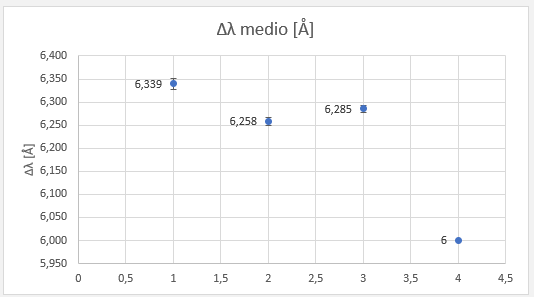
\includegraphics[width=0.6\linewidth]{IM grafico risultati delta lambda}
  \caption{Comparazione risultati $\Delta\lambda$}
\end{figure}


Come si può notare dai dati e dal grafico i nostri valori sono a diverse $\sigma$ di distanza dal valore vero. Ciò è causato dal fatto che l'errore considerato è solo quello strumentale calcolato con la formula:

\begin{equation} 
\sigma_{\Delta\lambda} = \sqrt{ (- \frac{n {\bar \lambda}^2}{2 \Delta X^2} \sigma_{\Delta X})^2} 
\end{equation}

L'errore predominante in questa misura è invece quello sulla lettura della posizione in cui scompaiono le fascie scure, dato che la transizione non è netta ma molto graduale.


Per aggirare il problema avremmo dovuto misurare più volte una posizione per ottenere l'errore statistico ma, a causa di una svista dello sperimentatore, ciò non è stato fatto. 

\vspace{3mm}

Riteniamo quindi di non poter eseguire alcuna analisi statistica per la compatibilità dei nostri valori rispetto al valore vero calcolato dai i valori forniti delle $\lambda$ emesse dalla lampada al sodio.




\section{Conclusioni}
Riteniamo i risultati ottenuti per la Misura 1 compatibili data la loro distanza di circa una deviazione standard dal valore vero. Per la Misura 2 ci limitiamo a considerare i valori plausibili data l'assenza di un valore con cui compararli. Per la Misura 3, non avendo nessun valore adatto alla comparazione, riteniamo che il risultato possa essere plausibile in comparazione al valore ottenuto dai nostri compagni e all'analisi fatta con il filtro verde ma riteniamo che il valore preciso possa essere errato data la grande incerteza. Per la Misura 4 ci limitiamo a riportare i dati senza un analisi statistica data la problematica dell'incertezza sulla misura di cui abbiamo discusso sopra.


\clearpage

\section{Appendice}
\subsection{Misura $\lambda$}

%immagine tabella lambda
\begin{figure}[h!]
  \centering
  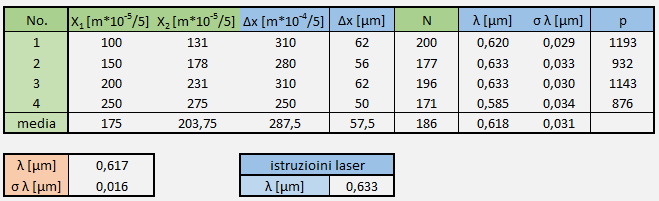
\includegraphics[width=1\linewidth]{IM tabella lambda}
  \caption{Tabella dati per il calcolo di $\lambda_{laser}$ e risultati}
\end{figure}


\subsection{Misura indice di rifrazione aria}


%Immagine tabella n
\begin{figure}[h!]
  \centering
  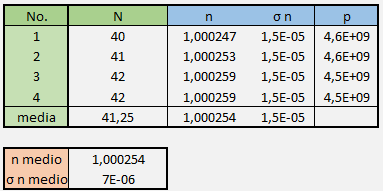
\includegraphics[width=0.6\linewidth]{IM tabella n}
  \caption{Tabella dati per il calcolo dell'indice di rifrazione aria e risultati}
\end{figure}

\subsection{Sistema $\lambda$-$n$}
\subsubsection{Sistema}

%Immagine tabelle sistema
\begin{figure}[h!]
  \centering
  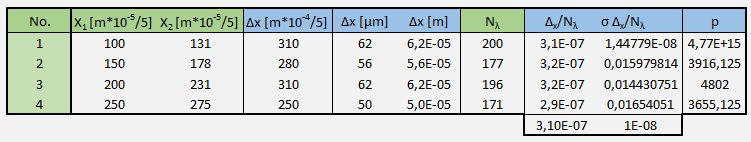
\includegraphics[width=1\linewidth]{IM tabella a}
  \caption{Tabella dati per il cacolo di a}
\end{figure}

\begin{figure}[h!]
  \centering
  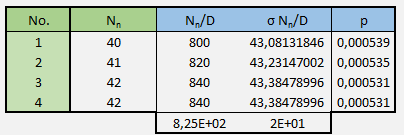
\includegraphics[width=0.6\linewidth]{IM tabella b}
  \caption{Tabella dati per il calcolo di b}
\end{figure}

\begin{figure}[h!]
  \centering
  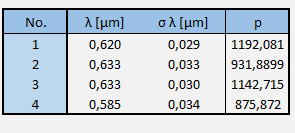
\includegraphics[width=0.4\linewidth]{IM tabella lambda sistema}
  \caption{Tabella per il calcolo di $\lambda$}
\end{figure}

\begin{figure}[h!]
  \centering
  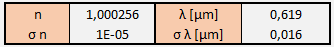
\includegraphics[width=0.6\linewidth]{IM risultati sistema}
  \caption{Risultati sistema}
\end{figure}
%fine tabelle sistema

\pagebreak 

\subsubsection{Metodo ricorsivo}

%tabella sistema ricorsivo
\begin{table}[h!]
\centering
\begin{tabular}{ | c | c | c | c | c | }
\hline
 $ricorsioni$ & $\lambda \; [\mu m]$ & $\sigma\lambda \; [\mu m]$ & $n$ & $\sigma n$\\
\hline
 1 & 0,618919207 & 0,015532975 & 1 & 0\\
 2 & 0,619077181 & 0,015536939 & 1,000255241 & 7,42201E-06\\
 3 & 0,619077221 & 0,01553694 & 1,000255306 & 7,4239E-06\\
 4 & 0,619077221 & 0,01553694 & 1,000255306 & 7,4239E-06\\
\hline
 $\Delta_{4 3}$ & -1,0292E-11 & -2,58319E-13 & -1,66287E-11 & 0\\
\hline
\end{tabular}
\caption{Risultati sistemi ricorsivo copiati dal foglio di calcolo}
\label{table:6}
\end{table}

\begin{figure}[h!]
  \centering
  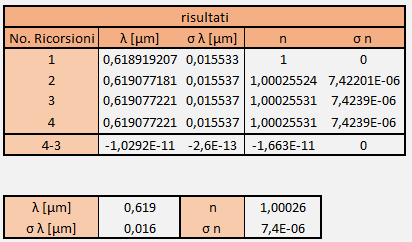
\includegraphics[width=0.6\linewidth]{IM tabella ricorsione}
  \caption{Tabella risultati del metodo ricorsivo parziali e finali}
\end{figure}


\pagebreak

\subsection{Misura pacchetto di luce bianca}

%tabella pacchetto
\begin{figure}[h!]
  \centering
  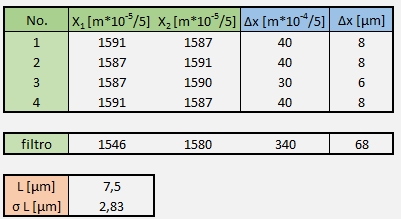
\includegraphics[width=0.6\linewidth]{IM tabella pacchetto}
  \caption{Tabella dati per il calcolo della lunghezza del pacchetto di luce bianca, dati filtro verde e risultati}
\end{figure}

\subsection{Misura $\Delta\lambda$ lampada al sodio}

%tabelle delta lambda
\begin{figure}[h!]
  \centering
  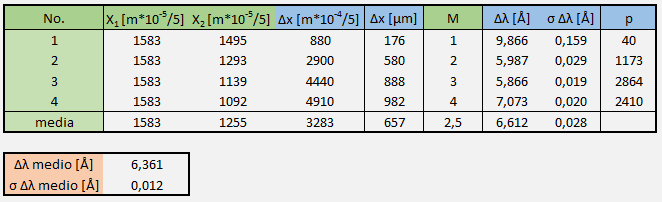
\includegraphics[width=0.75\linewidth]{IM tabella delta lambda set 1}
  \caption{Tabella dati per il calcolo di $\Delta\lambda$ e risultato parziale (set1)}
\end{figure}

\begin{figure}[h!]
  \centering
  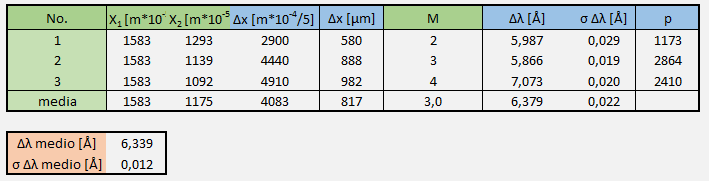
\includegraphics[width=0.75\linewidth]{IM tabella delta lambda set 1 scarto}
  \caption{Tabella dati per il calcolo di $\Delta\lambda$ dopo lo scarto e risultato parziale (set 1)}
\end{figure}

\begin{figure}[h!]
  \centering
  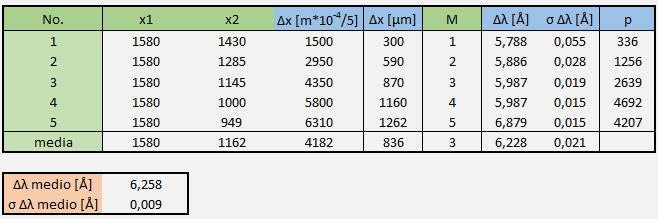
\includegraphics[width=0.75\linewidth]{IM tabella delta lambda set 2}
  \caption{Tabella dati per il calcolo di $\Delta\lambda$ e risultato parziale (set 2)}
\end{figure}

\begin{figure}[h!]
  \centering
  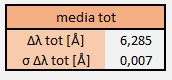
\includegraphics[width=0.25\linewidth]{IM risultati delta lambda}
  \caption{Risultato finale calcolo di $\Delta\lambda$}
\end{figure}
%fine tabelle delta lambda

\clearpage

\subsection{Comparazione risultati}

%inizio tabelle comparazione risultati
\begin{figure}[h!]
  \centering
  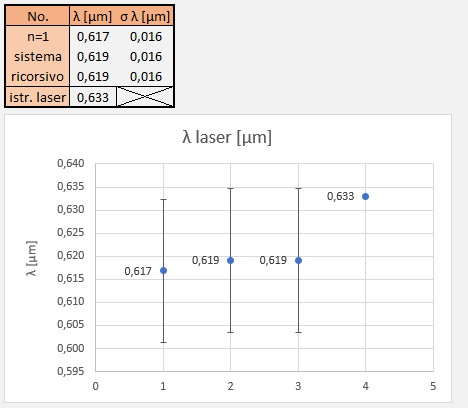
\includegraphics[width=0.6\linewidth]{IM comparazione lambda}
  \caption{Risultati e grafico di comparazione $\lambda$}
\end{figure}

\begin{figure}[h!]
  \centering
  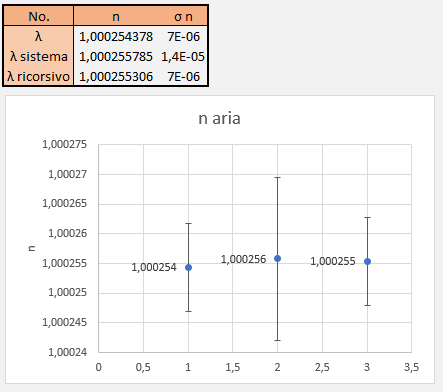
\includegraphics[width=0.6\linewidth]{IM comparazione n}
  \caption{Risultati e grafico di comparazione dell'indice di rifrazione dell'aria}
\end{figure}

\begin{figure}[h!]
  \centering
  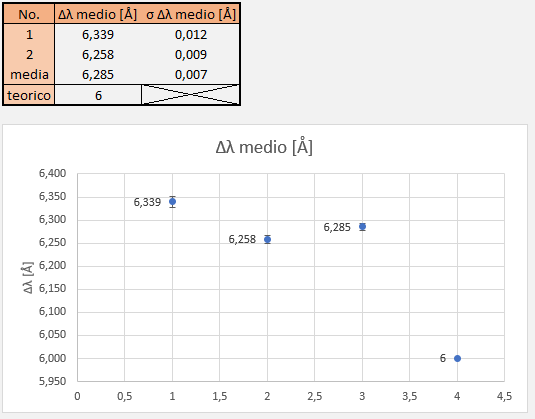
\includegraphics[width=0.6\linewidth]{IM comparazione delta lambda}
  \caption{Risultati e grafico di comparazione delle $\Delta\lambda$ della lampada al sodio}
\end{figure}

\end{document}